\section{Model Evaluation}


\begin{definition}{Model Evaluation}\\
Model evaluation is the process of assessing how well a machine learning model performs on unseen data. It helps us understand:
\begin{itemize}
    \item How accurate our predictions are
    \item Whether the model generalizes well to new data
    \item Which types of errors the model makes
    \item How to compare different models
\end{itemize}
\end{definition}

\subsubsection{Classification Evaluation}



\begin{definition}{Confusion Matrix}
The confusion matrix is a table that summarizes the performance of a classification model:
\begin{center}
\begin{tabular}{|c|c|c|}
\hline
$\downarrow y, \hat{y} \rightarrow$ & 1 & 0 \\
\hline
1 & TP=True Positive & FN=False Negative \\
\hline
0 & FP=False Positive & TN=True Negative \\
\hline
\end{tabular}
\end{center}
\end{definition}

\begin{definition}{Error Types}
\begin{itemize}
    \item \textbf{Type-I Error}: False-Positive (predicting positive when actual is negative)
    \item \textbf{Type-II Error}: False-Negative (predicting negative when actual is positive)
\end{itemize}
\end{definition}

\begin{formula}{Standard Error Measure}
$$E = \frac{1}{N}\sum_{i=1}^{N}(1 - id(\hat{y}_i, y_i))$$

where $id(a,b) = \begin{cases} 1 & \text{if } a = b \\ 0 & \text{else} \end{cases}$

Example: $datasize = 9$, $correct = 6$, $wrong = 3$
$$E = \frac{1}{9} \cdot 3 = 0.33$$
\end{formula}



\subsubsection{Performance Metrics}



\begin{formula}{Classification Metrics}
\begin{itemize}
    \item $A$ = Accuracy: Overall correctness (doesn't regard ''costs'' of errors)
    \item $R$ = Recall (Sensitivity): How many relevant cases have been found
    \item $P$ = Precision: How many of the found cases are relevant
    \item $F$ = F-Measure: Harmonic mean of recall and precision
\end{itemize}

$$A = \frac{TP + TN}{TP + TN + FP + FN}$$

$$R = \frac{TP}{TP + FN}$$

$$P = \frac{TP}{TP + FP}$$

$$F_1 = 2 \cdot \frac{R \cdot P}{R + P}$$
\end{formula}

\begin{definition}{Recall and Precision Interpretation}
$$Recall = \frac{relevant_{found}}{relevant_{total}}$$
$$Precision = \frac{relevant_{found}}{total_{found}}$$

Recall answers: Of all the positive cases, how many did we correctly identify?\\
Precision answers: Of all our positive predictions, how many were actually correct?
\end{definition}

\begin{center}
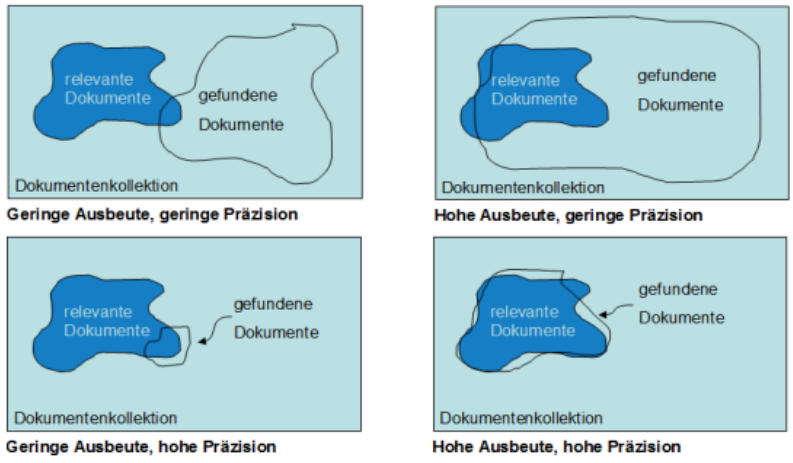
\includegraphics[width=0.8\linewidth]{precision_recall.png}
\end{center}


\begin{KR}{Choosing the Right Evaluation Metric}
\paragraph{Consider the problem context}
\begin{itemize}
    \item \textbf{Medical diagnosis}: High recall might be crucial (don't miss diseases)
    \item \textbf{Spam detection}: High precision might be important (don't flag important emails)
    \item \textbf{Balanced datasets}: Accuracy is often sufficient
    \item \textbf{Imbalanced datasets}: Focus on precision, recall, or F1-score
\end{itemize}

\paragraph{Balance precision and recall}
\begin{itemize}
    \item Use F1-score when you need a balance between precision and recall
    \item Consider F-beta score to weight precision or recall differently
    \item Plot precision-recall curves to see the trade-off
\end{itemize}
\end{KR}



\subsection{Advanced Evaluation Metrics}

\begin{formula}{Kappa Coefficient}\\
The Cohen's Kappa coefficient measures inter-rater agreement for categorical classifications:
\begin{itemize}
    \item $P(A)$ = proportion of agreements of the raters
    \item $P(E)$ = agreement, which we could get randomly
\end{itemize}

$$K = \frac{P(A) - P(E)}{1 - P(E)}$$

Interpretation:
\begin{itemize}
    \item $K = 1$: Perfect agreement
    \item $K = 0$: Agreement by chance
    \item $K < 0$: Worse than chance agreement
\end{itemize}
\end{formula}

\subsection{Model Fit Assessment}

\begin{concept}{Model Evaluation Patterns}
Three common patterns in model evaluation:
\begin{itemize}
    \item \textbf{Underfitted}: High bias, low variance - model is too simple
    \item \textbf{Good Fit/Robust}: Balanced bias and variance - optimal performance
    \item \textbf{Overfitted}: Low bias, high variance - model is too complex
\end{itemize}

Signs of overfitting:
\begin{itemize}
    \item High training accuracy but low test accuracy
    \item Large gap between training and validation performance
    \item Model performs poorly on new, unseen data
\end{itemize}

Signs of underfitting:
\begin{itemize}
    \item Low training and test accuracy
    \item Model cannot capture underlying patterns
    \item Adding more features or complexity improves performance
\end{itemize}
\end{concept}

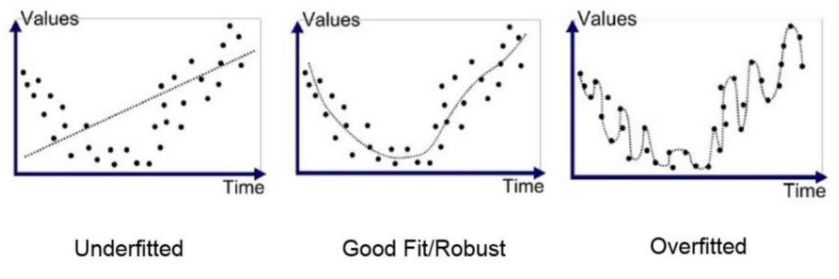
\includegraphics[width=\linewidth]{model_evaluation.png}
\subsection{Clustering Evaluation}

\begin{formula}{Silhouette Coefficient}\\
The Silhouette coefficient measures how well-separated clusters are:

$$s(i) = \frac{b(i) - a(i)}{\max(a(i), b(i))}$$

where:
\begin{itemize}
    \item $a(i)$ = average distance from point $i$ to other points in the same cluster
    \item $b(i)$ = average distance from point $i$ to points in the nearest cluster
\end{itemize}

Interpretation:
\begin{enumerate}
    \item $s \approx 1$: Sample is far away from neighboring clusters (good clustering)
    \item $s \approx 0$: Sample is close to the decision boundary between clusters
    \item $s \approx -1$: Sample might be assigned to the wrong cluster
\end{enumerate}
\end{formula}

\begin{concept}{Other Clustering Evaluation Metrics}
\begin{itemize}
    \item \textbf{Inertia (Within-cluster sum of squares)}: Measures compactness of clusters
    \item \textbf{Calinski-Harabasz Index}: Ratio of between-cluster to within-cluster variance
    \item \textbf{Davies-Bouldin Index}: Average similarity ratio of clusters
    \item \textbf{Adjusted Rand Index}: Measures similarity to ground truth clustering (if available)
\end{itemize}
\end{concept}

\subsection{Standardization and Normalization}

\begin{definition}{Standardization and Normalization}\\
    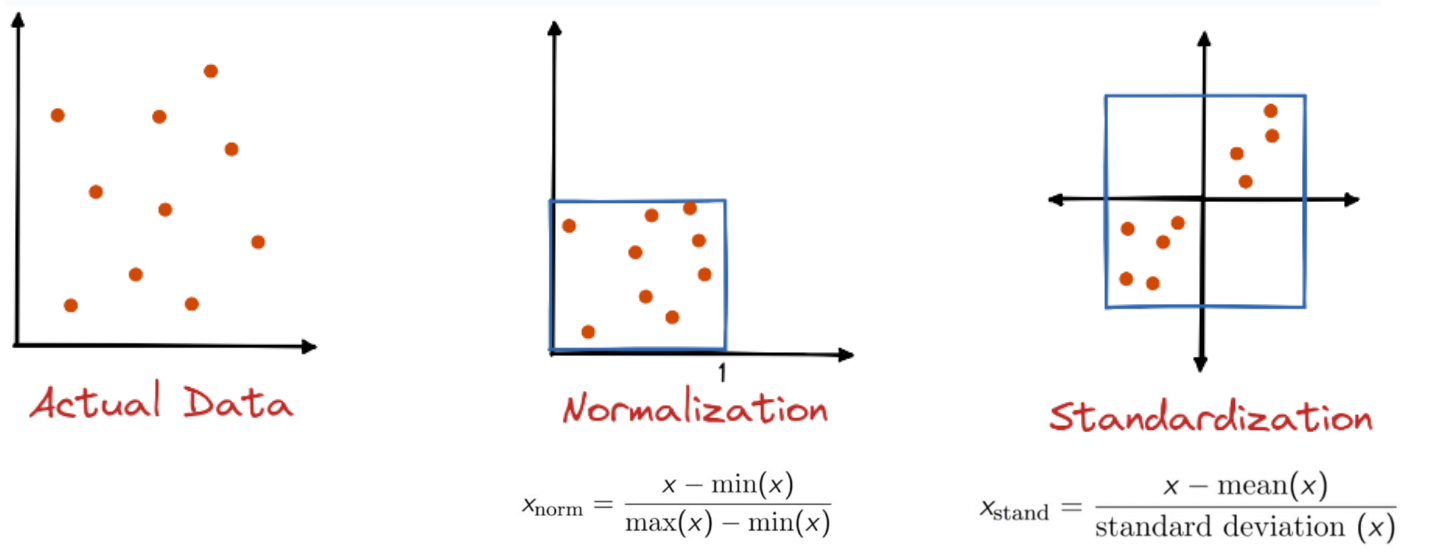
\includegraphics[width=\linewidth]{standardization_normalization.png}\\
    \small Normalization: e.g. for Neural Networks\\
    \small Standardization: e.g. for SVMs, Linear and Logistic Regression    
\end{definition}